
\textbf{Ejemplo 11}\newline
	Una aceptación bancaria por 80 millones COP con fecha de vencimiento el 17 de diciembre de 1999 es adquirida en 22 de julio de 1999 por un primer inversionista con una tasa del de 28\% período 28 días vencidos y es cedida a un segundo inversionista el 14 de octubre de 1999. Si el segundo inversionista desea ganarse el 32\% período días vencido utilice un año de 360 (año de 360 días) \\
	¿Cuál es la ganancia en pesos del primer inversionista? \\
	¿Cuál es la rentabilidad periódica días vencido del primer inversionista?\\

	\textbf{Solución.}
	\begin{center}

		\renewcommand{\arraystretch}{1.5}% Margenes de las celdas
		%Creación de la cuadricula
		\begin{longtable}[H]{|c|c|c| }
			%Creamos una linea horizontal
			\hline
			%Definimos el color de la primera fila
			\rowcolor[HTML]{FFB183}
			%%%%% INICIO ASIGNACIÓN FECHA FOCAL %%%%%%%
			%%%%%%%%%% INICIO TITULO
			%Lo que se hace aquí es mezclar las 3 columnas en una sola
			\multicolumn{3}{|c|}{\cellcolor[HTML]{FFB183}\textbf{1. Asignación período focal}}   \\ \hline
			%%%%%%%%%% FIN TITULO
			%%%%% INICIO DECLARACIÓN DE VARIABLES %%%%%%%
			\multicolumn{3}{|c|}{$pf = 0 pdv$} \\ \hline
			%Definimos el color de la primera fila
			\rowcolor[HTML]{FFB183}
			%%%%% INICIO DECLARACIÓN DE VARIABLES %%%%%%%
			%%%%%%%%%% INICIO TITULO
			\multicolumn{3}{|c|}{\cellcolor[HTML]{FFB183}\textbf{2. Declaración de variables}}                                                                                   \\ \hline
			%%%%%%%%%% FIN TITULO
			%%%%%%%%%% INICIO DE MATEMÁTICAS
			$i_{1} = 28 \% pdv$                                     & \multicolumn{2}{c|}{$ n_{1} = (145/365) pdv $} \\
			$i_{2} = 32\% pdv \hspace{0.3cm} $	& \multicolumn{2}{c|}{$ n_{2} = (63/365) pdv $} \\
			$P_{C2} - P_{C1} = ? $ & \multicolumn{2}{c|}{$ n_{3} = 0 pdv $}\\ \hline
			%%%%%%%%%% FIN DE MATEMÁTICAS
			%%%%% FIN DECLARACIÓN DE VARIABLES
			
			
			%%%%% INICIO FLUJO DE CAJA
			\rowcolor[HTML]{FFB183}
			\multicolumn{3}{|c|}{\cellcolor[HTML]{FFB183}\textbf{3. Diagrama de flujo de caja}}                                                                                  \\ \hline
			%Mezclamos 3 columnas y pondremos el dibujo
			%%%%%%%%%%%%% INSERCIÓN DE LA IMAGEN
			\multicolumn{3}{|c|}{ 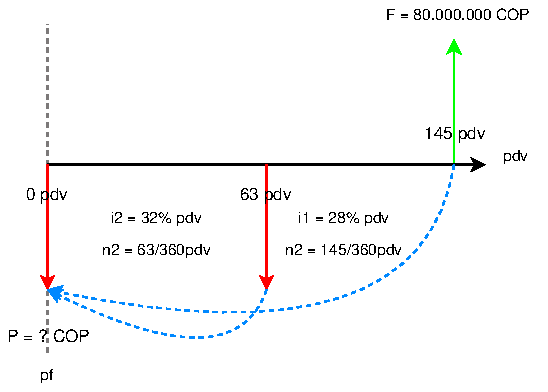
\includegraphics[trim=-78 -5 -78 -5]{3_Capitulo/img/ejemplos/11/capitulo3ejercicio11.pdf} }                                                                                         \\ \hline
			%%%%%%%%%%%%% FIN INSERCIÓN DE IMAGEN
			%%%%%FIN FLUJO DE CAJA
			
			
			
			%%%%% INICIO DECLARACIÓN FORMULAS
			%%%%%%%%%%% INICIO TITULO
			\rowcolor[HTML]{FFB183}
			\multicolumn{3}{|c|}{\cellcolor[HTML]{FFB183}\textbf{4. Declaración de fórmulas}}                                                                                    \\ \hline
			%%%%%%%%%%% FIN TITULO
			%%%%%%%%%%% INICIO MATEMÁTICAS
		
			 \multicolumn{3}{|c|}{$P=F(1+i    )^{-n}$\hspace{35pt}\textit{Valor presente}\hspace{0.3cm}}\\ \hline
			%%%%%%%%%% FIN MATEMÁTICAS
			%%%%%% INICIO DESARROLLO MATEMÁTICO
			\rowcolor[HTML]{FFB183}
			%%%%%%%%%%INICIO TITULO
			\multicolumn{3}{|c|}{\cellcolor[HTML]{FFB183}\textbf{5. Desarrollo matemático}}                                                                                      \\ \hline
			%%%%%%%%%% FIN TITULO
			%%%%%%%%%% INICIO MATEMÁTICAS
			\multicolumn{3}{|c|}{$Pc_1 =   80{.}000{.}000 COP (1+0,28)\frac{-145}{360}$ =   72{.}428{.}283,64 COP $\simeq$   72{.}428{.}284 COP \hspace{3pt}\textit{Ecuación de valor}}
			\\ 
			\multicolumn{3}{|c|}{$Pc_2 =   80{.}000{.}000 COP(1+0,32)\frac{-63}{360} =    76{.}206{.}067 COP$ \hspace{3pt}\textit{Ecuación de valor}}
			\\ 
			\multicolumn{3}{|c|}{$Pc_1 =  P_{C2} - P_{C1} COP  = 76{.}206{.}067 - 72{.}428{.}284  =   3{.}777{.}738 COP  $ \hspace{3pt}\textit{Ecuación de valor}}
			                             \\ \hline
			%%%%%%%%%% FIN MATEMÁTICAS
			%%%%%% FIN DESARROLLO MATEMÁTICO
			
			\rowcolor[HTML]{FFB183}
			\multicolumn{3}{|c|}{\cellcolor[HTML]{FFB183}\textbf{6. Respuesta}}    \\ \hline    
			
			\multicolumn{3}{|c|}{$P_{C2} - P_{C1} =  3{.}777{.}783 COP  $} \\ \hline
		\end{longtable}
		%Se crean dos lineas en blanco para que no quede el siguiente texto tan pegado
	\end{center}

%%%%%%%%%%%%%%%%%%%%%%%%%%FIN EJERCICIO X %%%%%%%%%%%%%%%%%%%%%%%%%%%